% Created 2020-09-10 Thu 17:06
% Intended LaTeX compiler: pdflatex
\documentclass[unicode, 12pt, aspectratio=43]{beamer}
\usepackage[utf8]{inputenc}
\usepackage[T1]{fontenc}
\usepackage{graphicx}
\usepackage{grffile}
\usepackage{longtable}
\usepackage{wrapfig}
\usepackage{rotating}
\usepackage[normalem]{ulem}
\usepackage{amsmath}
\usepackage{textcomp}
\usepackage{amssymb}
\usepackage{capt-of}
\usepackage{hyperref}
\usepackage[backend=bibtex, style=authortitle]{biblatex}
\AtEveryCitekey{\iffootnote{\tiny\reffont}{\color{blue}}}
\addbibresource{../resources/anthology.bib}
\addbibresource{../resources/my.bib}
\usepackage{url}
\usetheme{metropolis}
\setbeamertemplate{footline}{ \hfill \usebeamercolor[fg]{page number in head/foot} \usebeamerfont{page number in head/foot} \insertframenumber\kern1em\vskip2pt }
\setbeamertemplate{items}[default]
\setbeamertemplate{itemize item}{\small\raise0.5pt\hbox{$\blacksquare$}}
\setbeamertemplate{itemize subitem}{\footnotesize\raise1.5pt\hbox{$\bullet$}}
\setbeamertemplate{itemize subsubitem}{\scriptsize\raise1.5pt\hbox{$\blacktriangleright$}}
\setbeamertemplate{navigation symbols}{}
\usepackage{xltxtra}
\usepackage{booktabs}
\usepackage[absolute,overlay]{textpos}
\usepackage{pgfpages}
\usefonttheme{professionalfonts}
\usepackage[T1]{fontenc}
\usepackage{fontspec}
\XeTeXlinebreaklocale "ja"
\setsansfont[AutoFakeSlant=0.2]{Noto Sans CJK JP}
\setromanfont[AutoFakeSlant=0.2]{Noto Serif CJK JP}
\newfontfamily\emojifont{Noto Emoji}
\newfontfamily\octicons{github-octicons}
\newfontfamily\materials{Material Icons}
\newfontfamily\reffont{Times New Roman}
\renewcommand{\baselinestretch}{1.3}
\usetheme{default}
\author{出口 祥之 \\ \lower2.0pt\hbox{\materials} \texttt{deguchi@ai.cs.ehime-u.ac.jp}}
\date{2020/07/30 二宮研 論文輪読会}
\title{Dynamic Programming Encoding for Subword Segmentation in Neural Machine Translation}
\subtitle{(He et al., ACL 2020)}
\institute{}
\hypersetup{
 pdfauthor={出口 祥之 \\ \lower2.0pt\hbox{\materials} \texttt{deguchi@ai.cs.ehime-u.ac.jp}},
 pdftitle={Dynamic Programming Encoding for Subword Segmentation in Neural Machine Translation},
 pdfkeywords={},
 pdfsubject={},
 pdfcreator={Emacs 27.1 (Org mode 9.3.7)}, 
 pdflang={English}}
\begin{document}

\maketitle

\begin{frame}[label={sec:org58e037a}]{\hbox{\octicons} Links}
\begin{block}{\raise0.5pt\hbox{\octicons} Paper}
\begin{block}{\url{https://www.aclweb.org/anthology/2020.acl-main.275/}}
\end{block}
\end{block}
\begin{block}{\raise0.5pt\hbox{\octicons} Source Code}
\begin{block}{\url{https://github.com/xlhex/dpe}}
\end{block}
\end{block}
\end{frame}

\begin{frame}[label={sec:orgd35ce31}]{Introduction}
\begin{block}{NMT におけるサブワード分割}
\begin{description}
\item[{貪欲法:}] バイトペア符号化 (BPE)\footcite{sennrich-etal-2016-neural}, 最長一致法\footcite{wu-etal-2016-googles}
\item[{確率的アルゴリズム:}] ユニグラムLM\footcite{kudo-2018-subword}, BPE-dropout\footcite{provilkov-etal-2020-bpe}
\item \small 原言語側,目的言語側ともに複数分割候補が得られる.訓練時に分割候補を確率的にサンプリングすることでモデルの頑健性向上. \normalsize
\item[{動的計画法:}] 提案手法.サブワード分割の周辺化.
\end{description}
\end{block}
\end{frame}

\begin{frame}[label={sec:org2e8f372}]{Related Work (Greedy Algorithms)}
\begin{block}{BPE, Wordpiece}
\begin{itemize}
\item unconscious \(\rightarrow\) un + conscious, likes \(\rightarrow\) like + s
\item 隣り合った頻出サブワードから順に,予め指定した語彙数に到達するまで再帰的に結合 (BPE)
\item 語彙数とデコード速度はトレードオフ
\begin{itemize}
\item (語彙数を小さくするだけであれば文字単位でよい)
\item テキスト圧縮の技術を利用
\item 語彙数の上限を制約とし,文長が短くなるような分割を得るアルゴリズム
\end{itemize}
\end{itemize}
\end{block}
\end{frame}

\begin{frame}[label={sec:orgf51776a}]{Related Work (Stochastic Algorithms)}
\begin{block}{ユニグラムLM, BPE-dropout}
\begin{itemize}
\item \footnotesize unconscious \(\rightarrow\) \{un + concious, uncon + scious\}
\item \normalsize 複数分割候補を得られる
\begin{itemize}
\item ユニグラムLM: 尤度ベースでサンプリング
\item BPE-dropout: 結合時に確率的に棄却
\item NMT 訓練時に分割を確率的に得ることでデータ拡張 (Data Augumentation) の効果
\begin{itemize}
\item モデルの頑健性,汎用化
\end{itemize}
\end{itemize}
\end{itemize}
\end{block}
\end{frame}

\begin{frame}[label={sec:orgb050160}]{\normalsize Related Work (Dynamic Programming Algorithms)}
\begin{block}{音声認識\footcite{wang-etal-2017-sequence}}
\end{block}

\begin{block}{非自己回帰 NMT モデル\footcite{chan-etal-2020-imputer}\footcite{saharia-etal-2020-nonautoregressive}}
\end{block}
\end{frame}

\begin{frame}[label={sec:orgcfeb290}]{Latent Subword Segmentation - Definitions}
\begin{block}{\hspace{-0.75cm}目的言語側の分割を潜在変数とみなす}
\begin{columns}
\begin{column}{1.0\columnwidth}
\begin{itemize}
\item \(M\) 個のサブワード境界: \(\{\boldsymbol{y}_{z_i, z_{i+1}}\}_{i=1}^M\)
\begin{itemize}
\item \(\boldsymbol{y} = (y_1, \ldots, y_T)\): 目的言語文の文字列
\item \(\boldsymbol{z} = (z_1 (=0),\ldots,z_{M+1} (=T))\): 文字インデックス列
\item \(\boldsymbol{y}_{a,b}\): \((a+1)^\text{th}\) から \(b^\text{th}\) まで結合したサブワード
\end{itemize}
\end{itemize}
\end{column}

\begin{column}{0.465\columnwidth}
\begin{textblock*}{\linewidth}(220pt, 40pt)
    \centering
    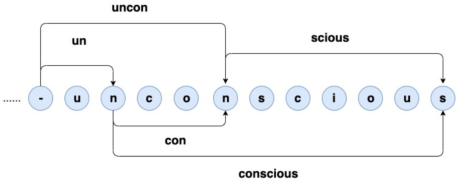
\includegraphics[width=\linewidth]{./figure/Figure1.pdf}
\end{textblock*}
\end{column}
\end{columns}
\end{block}

\begin{columns}
\begin{column}{0.5\columnwidth}
\begin{block}{例:}
\footnotesize
\begin{itemize}
\item 辞書 \(\mathcal{V} = \{\text{'c', 'a', 't', 'ca', 'at'}\}\)
\item 単語: 'cat'
\end{itemize}
\end{block}
\end{column}

\begin{column}{0.5\columnwidth}
\footnotesize

\begin{center}
\begin{tabular}{ll}
\toprule
\(\boldsymbol{z}\) & サブワード列\\
\midrule
\((0,1,3)\) & ('c', 'at')\\
\((0,2,3)\) & ('ca', 't')\\
\((0,1,2,3)\) & ('c', 'a', 't')\\
\bottomrule
\end{tabular}
\end{center}
\end{column}
\end{columns}
\end{frame}

\begin{frame}[label={sec:orged48bc1}]{Latent Subword Segmentation - Likelihood}
\begin{block}{連鎖律を用いてサブワード列の対数尤度を表現}
\begin{itemize}
\item 各サブワードにおいて語彙のカテゴリ分布を生成
\begin{equation*}
  \log p(\boldsymbol{y},\boldsymbol{z} | \boldsymbol{x}) = \sum_{i=1}^{|\boldsymbol{z}|} \log p(\boldsymbol{y}_{z_i, z_{i+1}} | \boldsymbol{y}_{z_1, z_2},\ldots,\boldsymbol{y}_{z_{i-1}, z_i}, \boldsymbol{x})
\end{equation*}
※ \(\boldsymbol{x}\) : 原言語文
\item 殆どの NMT は \(\boldsymbol{z}\) は \(\boldsymbol{y}\) の決定論的関数とみなされる: \(\log p(\boldsymbol{y}, \boldsymbol{z}) \approx \log p(\boldsymbol{y})\)
\end{itemize}
\end{block}
\end{frame}

\begin{frame}[label={sec:org68c6bda}]{\normalsize Latent Subword Segmentation - Latent Variable}
\begin{block}{\(\boldsymbol{z} \in \mathcal{Z}_{y} (\boldsymbol{y} \text{の分割集合})\) を潜在表現とみなす}
\begin{itemize}
\item \(p(\boldsymbol{y} | \boldsymbol{x}) = \sum_{\boldsymbol{z}} p(\boldsymbol{y}, \boldsymbol{z} | \boldsymbol{x})\) とする
\begin{equation*}
  \small \log p(\boldsymbol{y} | \boldsymbol{x}) = \log\sum_{\boldsymbol{z}\in\mathcal{Z}_y}\exp\sum_{i=1}^{|\boldsymbol{z}|} \log p(\boldsymbol{y}_{z_i, z_{i+1}} | \boldsymbol{y}_{z_1, z_2},\ldots,\boldsymbol{y}_{z_{i-1}, z_i}, \boldsymbol{x})
\end{equation*}
※ 対数周辺尤度の下限: \(\log p(\boldsymbol{y} | \boldsymbol{x}) \ge \log p(\boldsymbol{y}, \boldsymbol{z} | \boldsymbol{x})\)

\item 各サブワードの確率が条件部のコンテキストの分割に依存するため,巨大な空間 \(\mathcal{Z}_y\) 上での厳密な周辺化は組み合わせ爆発を起こす
\end{itemize}
\end{block}
\end{frame}

\begin{frame}[label={sec:org0f3add6}]{A Mixed Character-Subword Transformer}
\begin{block}{文字に基づいてサブワードを生成する Transformer}
\begin{itemize}
\item 条件部のコンテキストを文字のみに
\begin{equation*}
  \log p(\boldsymbol{y}, \boldsymbol{z} | \boldsymbol{x}) = \sum_{i=1}^{|\boldsymbol{z}|} \log p(\boldsymbol{y}_{z_i, z_{i+1}} | y_{z_1}, \ldots, y_{z_i}, \boldsymbol{x})
\end{equation*}

\item \(\boldsymbol{y}\) の各文字位置 \(t\) において,次に来るサブワード \(w \in \mathcal{V}\) の分布を以下に基づいて生成
\begin{equation*}
  p(w | y_{1}, \ldots, y_{t}, \boldsymbol{x}) = \frac{\exp(f(y_1,\ldots,y_t)^\top e(w))}{\sum_{w' \in \mathcal{V}}\exp(f(y_1,\ldots,y_t)^\top e(w'))}
\end{equation*}
\begin{itemize}
\item \vspace{-0.5cm} \(f(\cdot)\) : Transformer により条件部の計算
\item \(e(\cdot)\) : ソフトマックス層の重み
\end{itemize}
\end{itemize}
\end{block}
\end{frame}

\begin{frame}[label={sec:org70502e6}]{A Mixed Character-Subword Transformer}
\begin{columns}
\begin{column}{0.65\columnwidth}
\begin{block}{\(t\) ステップ目のモデル出力}
\begin{enumerate}
\item \(t\) ステップ目でサブワード \(w\) を生成
\item サブワード \(w\) の文字をデコーダに入力 ( \(t+1\) から \(t+|w|\) まで )
\item \(t+|w|\) ステップ目で次のサブワードを生成
\end{enumerate}
\end{block}
\end{column}

\begin{column}{0.35\columnwidth}
\begin{center}
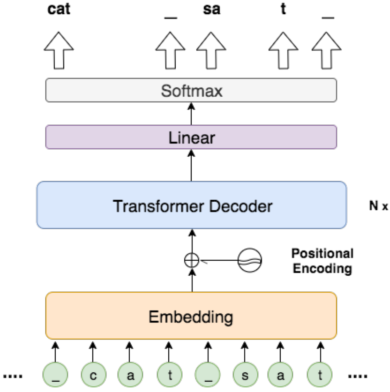
\includegraphics[width=\linewidth]{./figure/Figure2.pdf}
\end{center}
\end{column}
\end{columns}
\end{frame}

\begin{frame}[label={sec:org6b1f2eb}]{Optimization}
\begin{block}{目的関数 \(\mathcal{L}(\theta)\) を最大化}
\begin{equation*}
  \mathcal{L}(\theta) = \sum_{(\boldsymbol{x}, \boldsymbol{y}) \in \mathcal{D}} \log P(\boldsymbol{y} | \boldsymbol{x})
\end{equation*}
\begin{itemize}
\item 周辺化と対数周辺尤度の勾配計算が必要
\end{itemize}
\end{block}
\end{frame}

\begin{frame}[label={sec:org87578a8}]{Exact Maginalization}
\begin{block}{動的計画法を用いて周辺尤度を計算}
\begin{itemize}
\item サブワードの出力確率が文字のみによって得られるため動的計画法によって対数周辺尤度が計算可能
\end{itemize}
\begin{center}
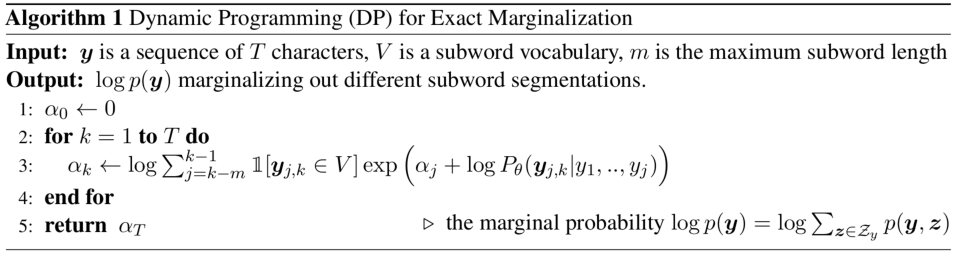
\includegraphics[width=\linewidth]{./figure/Algorithm1.pdf}
\end{center}
\begin{itemize}
\item 計算量:  \(\mathcal{O}(mT)\)
\begin{itemize}
\item \(m\) : 語彙に含まれる最長の単語の文字数
\end{itemize}
\end{itemize}
\end{block}
\end{frame}

\begin{frame}[label={sec:orgabc43e6}]{Gradient Computation}
\begin{block}{計算量増加への対処}
\begin{itemize}
\item PyTorch での著者実装で通常の Transformer デコーダより 8 倍遅く,メモリ使用量も増加
\begin{itemize}
\item DP アルゴリズムと文字レベルでの演算による系列長の増加が原因
\end{itemize}
\item Transformer のレイヤ数を 6 から 4 に減らし,16 ステップ勾配蓄積 (Gradient Accumulattion) してからパラメタ更新
\end{itemize}
\end{block}
\end{frame}

\begin{frame}[label={sec:orga2672eb}]{Segmenting Target Sentences}
\begin{block}{Dynamic Programming Encoding (DPE): 最大事後確率を持つ目的言語文の分割を探索}
\begin{center}
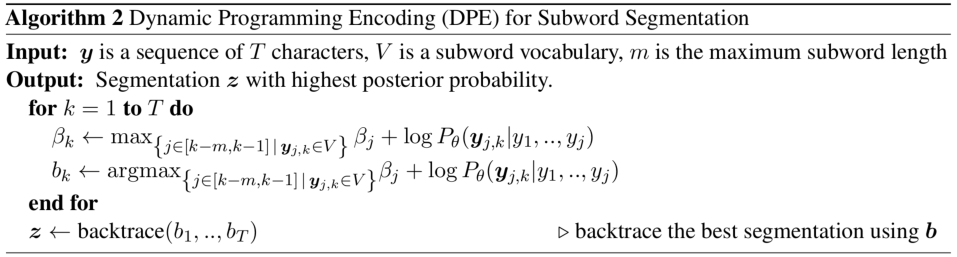
\includegraphics[width=\linewidth]{./figure/Algorithm2.pdf}
\end{center}
\end{block}
\end{frame}

\begin{frame}[label={sec:org9b9b696}]{Segmenting Target Sentences}
\begin{itemize}
\item 混合文字サブワード Transformer は訓練データの目的言語文の分割のためのみに使用
\item 分割した文で通常のサブワード Transformer を訓練
\end{itemize}
\begin{center}
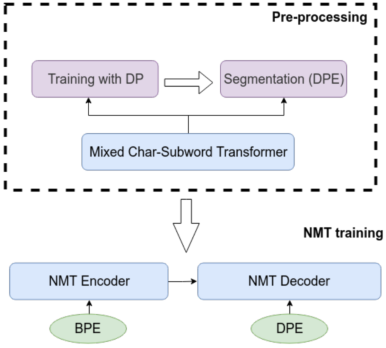
\includegraphics[width=0.5\linewidth]{./figure/Figure3.pdf}
\end{center}
\end{frame}

\begin{frame}[label={sec:orgca68eed}]{Experiments}
\begin{description}
\item[{データセット}] WMT09 En-Hu, WMT14 En-De, WMT15 En-Fi, WMT16 En-Ro, WMT18 En-Et
\item[{モデル}] 
\end{description}
\begin{center}
\begin{tabular}{ll}
\toprule
アーキテクチャ & Transformer base\\
分割 (原言語側) & BPE-dropout \((p=0.05)\)\\
   (目的言語側) & DPE\\
\bottomrule
\end{tabular}
\end{center}
\end{frame}

\begin{frame}[label={sec:orgeacdf02}]{Main Results}
\begin{center}
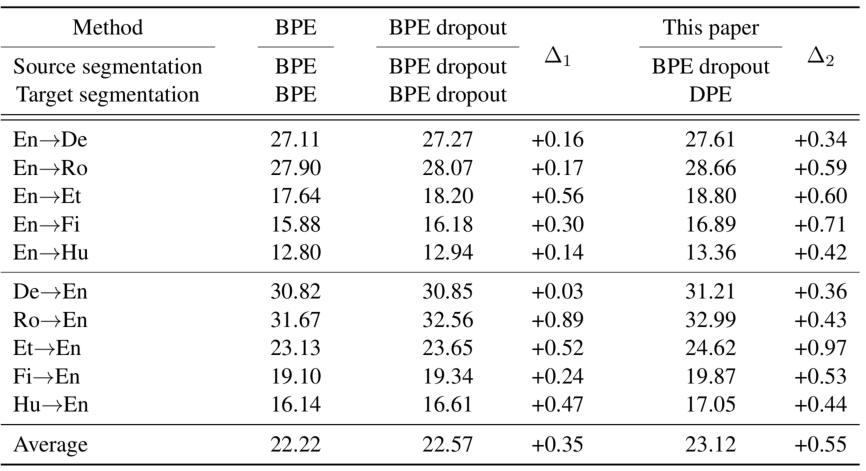
\includegraphics[width=\linewidth]{./figure/Table2.pdf}
\end{center}
\end{frame}

\begin{frame}[label={sec:org84c2519}]{Segmentation Examples}
\begin{center}
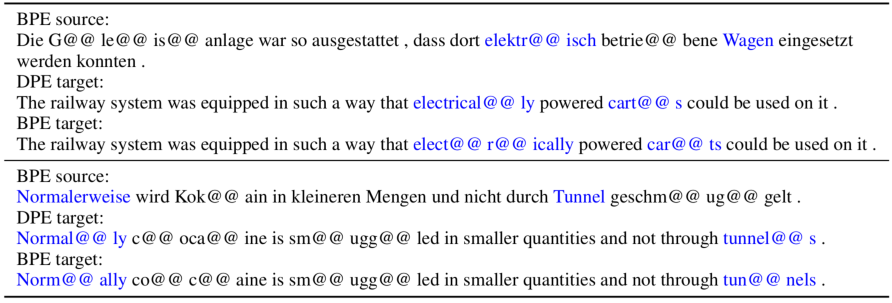
\includegraphics[width=\linewidth]{./figure/Table3.pdf}
\end{center}
\begin{itemize}
\item 他の例は論文参照
\end{itemize}
\end{frame}

\begin{frame}[label={sec:org5758021}]{Conditional Subword Segmentation}
\begin{block}{原言語文を条件部に入れず,LM で分割}
\begin{center}
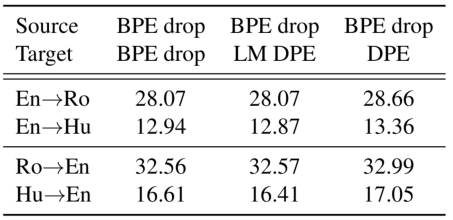
\includegraphics[width=0.4\linewidth]{./figure/Table5.pdf}
\end{center}
\end{block}

\begin{block}{同一の目的言語文で原言語側を変えて違いを比較}
\begin{center}
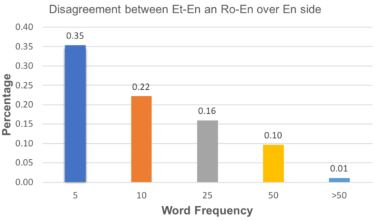
\includegraphics[width=0.45\linewidth]{./figure/Figure4.pdf}
\end{center}
\end{block}
\end{frame}

\begin{frame}[label={sec:orge9c4dc3}]{Conditional Subword Segmentation}
\begin{block}{\small 原言語文が BPE-dropout によって変化することの有効性}
\begin{center}
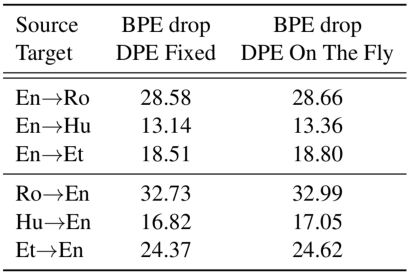
\includegraphics[width=0.5\linewidth]{./figure/Table6.pdf}
\end{center}
\end{block}
\end{frame}

\begin{frame}[label={sec:org8b33e17}]{DPE vs BPE}
\begin{block}{目的言語側の分割アルゴリズムを変えて比較}
\begin{center}
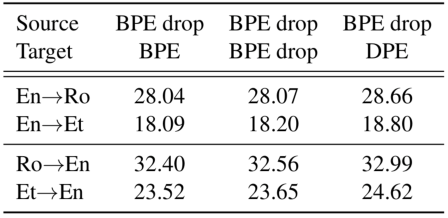
\includegraphics[width=0.5\linewidth]{./figure/Table7.pdf}
\end{center}
\end{block}
\end{frame}

\begin{frame}[label={sec:org09324f5}]{Conclusion}
\begin{itemize}
\item \textbf{Dynamic Programming Encoding} を提案
\begin{itemize}
\item 訓練時は目的言語側の分割を潜在変数とみなして周辺化
\item 推論時は事後確率が最も高くなる分割を出力
\end{itemize}
\item BPE だけでなく BPE-dropout と比較しても翻訳性能が向上
\end{itemize}
\end{frame}
\end{document}